\documentclass[a4paper,12pt]{article} 
\usepackage{ctex,abstract,graphicx}
\usepackage{subfigure,float}
\usepackage[a4paper, total={6in, 8in}]{geometry}

\begin{document}

\title {杭州出游}
\author{My Name}
\date{\today}
\maketitle

\pagenumbering{Roman}
\renewcommand{\abstractname}{\textbf{\zihao{4}摘\quad 要}}
\begin{onecolabstract}
  本文对杭州出行的意义作了分析,其中主要聚焦于解决为什么要出游这一问题。同时分析了杭州景点、交通
  和文化意义。并给出了可行的方案。

  
  \addcontentsline{toc}{section}{摘要}\tolerance=500 % 将摘要添加到目录中

  \noindent{\textbf{关键词:}杭州、乐观、文化}
\end{onecolabstract}
\renewcommand{\abstractname}{\textbf{Abstract}}
\begin{onecolabstract}
  TThis article analyzes the significance of traveling in Hangzhou, 
  with a focus on solving the problem of why one needs to travel. Simultaneously ana
  lyzed Hangzhou's scenic spots and transportation 
  and cultural significance. And feasible solutions were provided.

  \noindent{\textbf{Keywords:}Hangzhou, Optimistic, Culture}
\end{onecolabstract}
\newpage
\begin{center}
  \tableofcontents
\end{center}


\newpage
\pagenumbering{arabic}

\section{绪论}
  !!划重点:这是一个即将开学的某大学生为熟悉论文、计算机以及tex等等所作,部分成果还需要进一步考证

  众所周知,现在的大学生学业繁重,部分学生群体精神状态不好,需要出行来缓解压力。这些特征,在三本尤为明显,有以下图片证明。
  \begin{figure}[htbp]
    \centering
    \subfigure[Proof one]{
    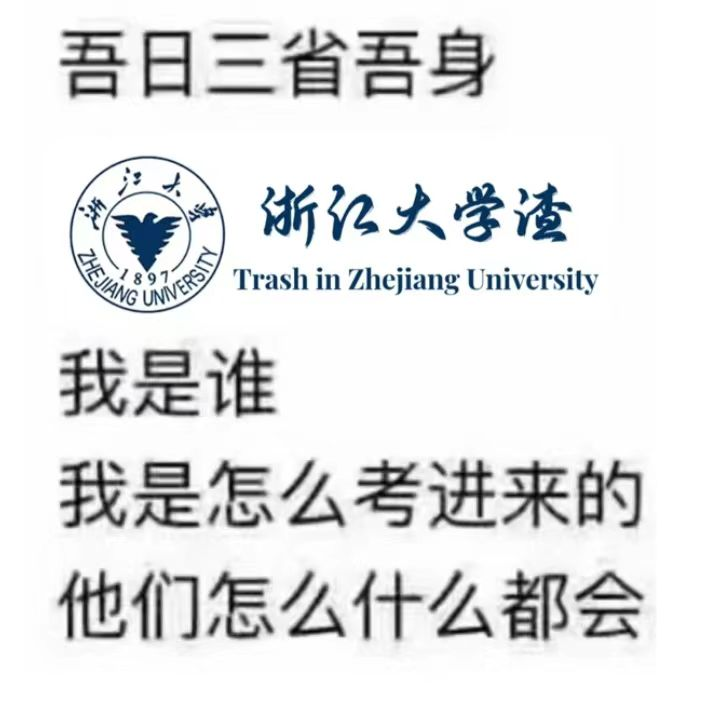
\includegraphics[scale=0.25]{1.jpg} \label{1}
    }
    \quad
    \subfigure[Proof two]{
    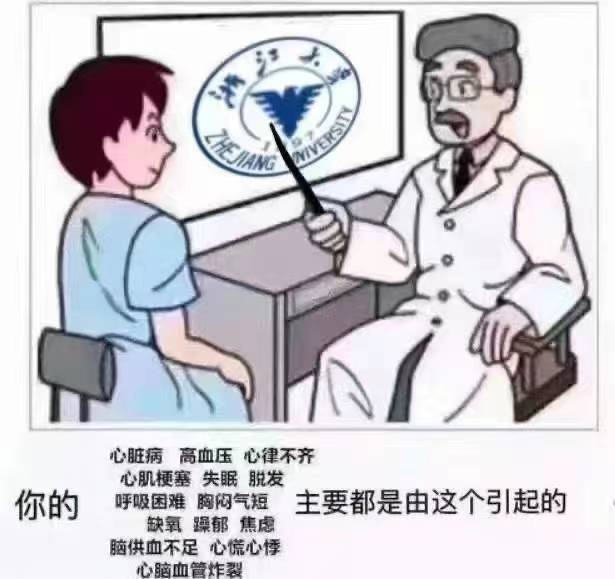
\includegraphics[scale=0.25]{2.jpg} \label{2} 
    }
    
    \caption{Experimental results of the author}
    \end{figure}

  所以,为了我们能够更好的学习,根据不同文献的观点和结论,得出结论:学生可以通过出游,实现

  1.放松心情,见证自然的美好;

  2.以更加积极的心态投入学习。

  但是,杭州人口众多,在许多地方人山人海,游玩并不便利。其次,学生们不清楚哪里有趣,哪里的饭好吃。由此,催生了本次研究。
  

\subsection{研究背景}
人人都说江南好,我却最爱是杭城,细雨缠绵,晨曦微漾,杭州总是充满了风雅与恬静。

(以下为AI所写)杭州作为江南水乡的代表,以其独特的风景和文化魅力吸引着无数游客。细雨缠绵的江南水乡气息,晨
曦微漾的西湖美景,让人仿佛置身于一幅幽静而优美的画卷中。杭州不仅有着自然风光的优美,还有着悠久的历史文化和
独特的传统饮食,使人沉浸其中无法自拔。

在杭州,古老的灵隐寺传承着千年的佛教文化,西湖边的雷峰塔见证着历史的变迁,南宋御街保留着古老的街道风貌,每
一处景点都散发着浓厚的历史气息。而杭州的龙井茶、西湖醋鱼、宋嫂鱼羹等美食更是让人流连忘返,品尝美食的同
时体验着当地的饮食文化。

\begin{figure}[htbp]
  \centering
  \subfigure[Example one]{
  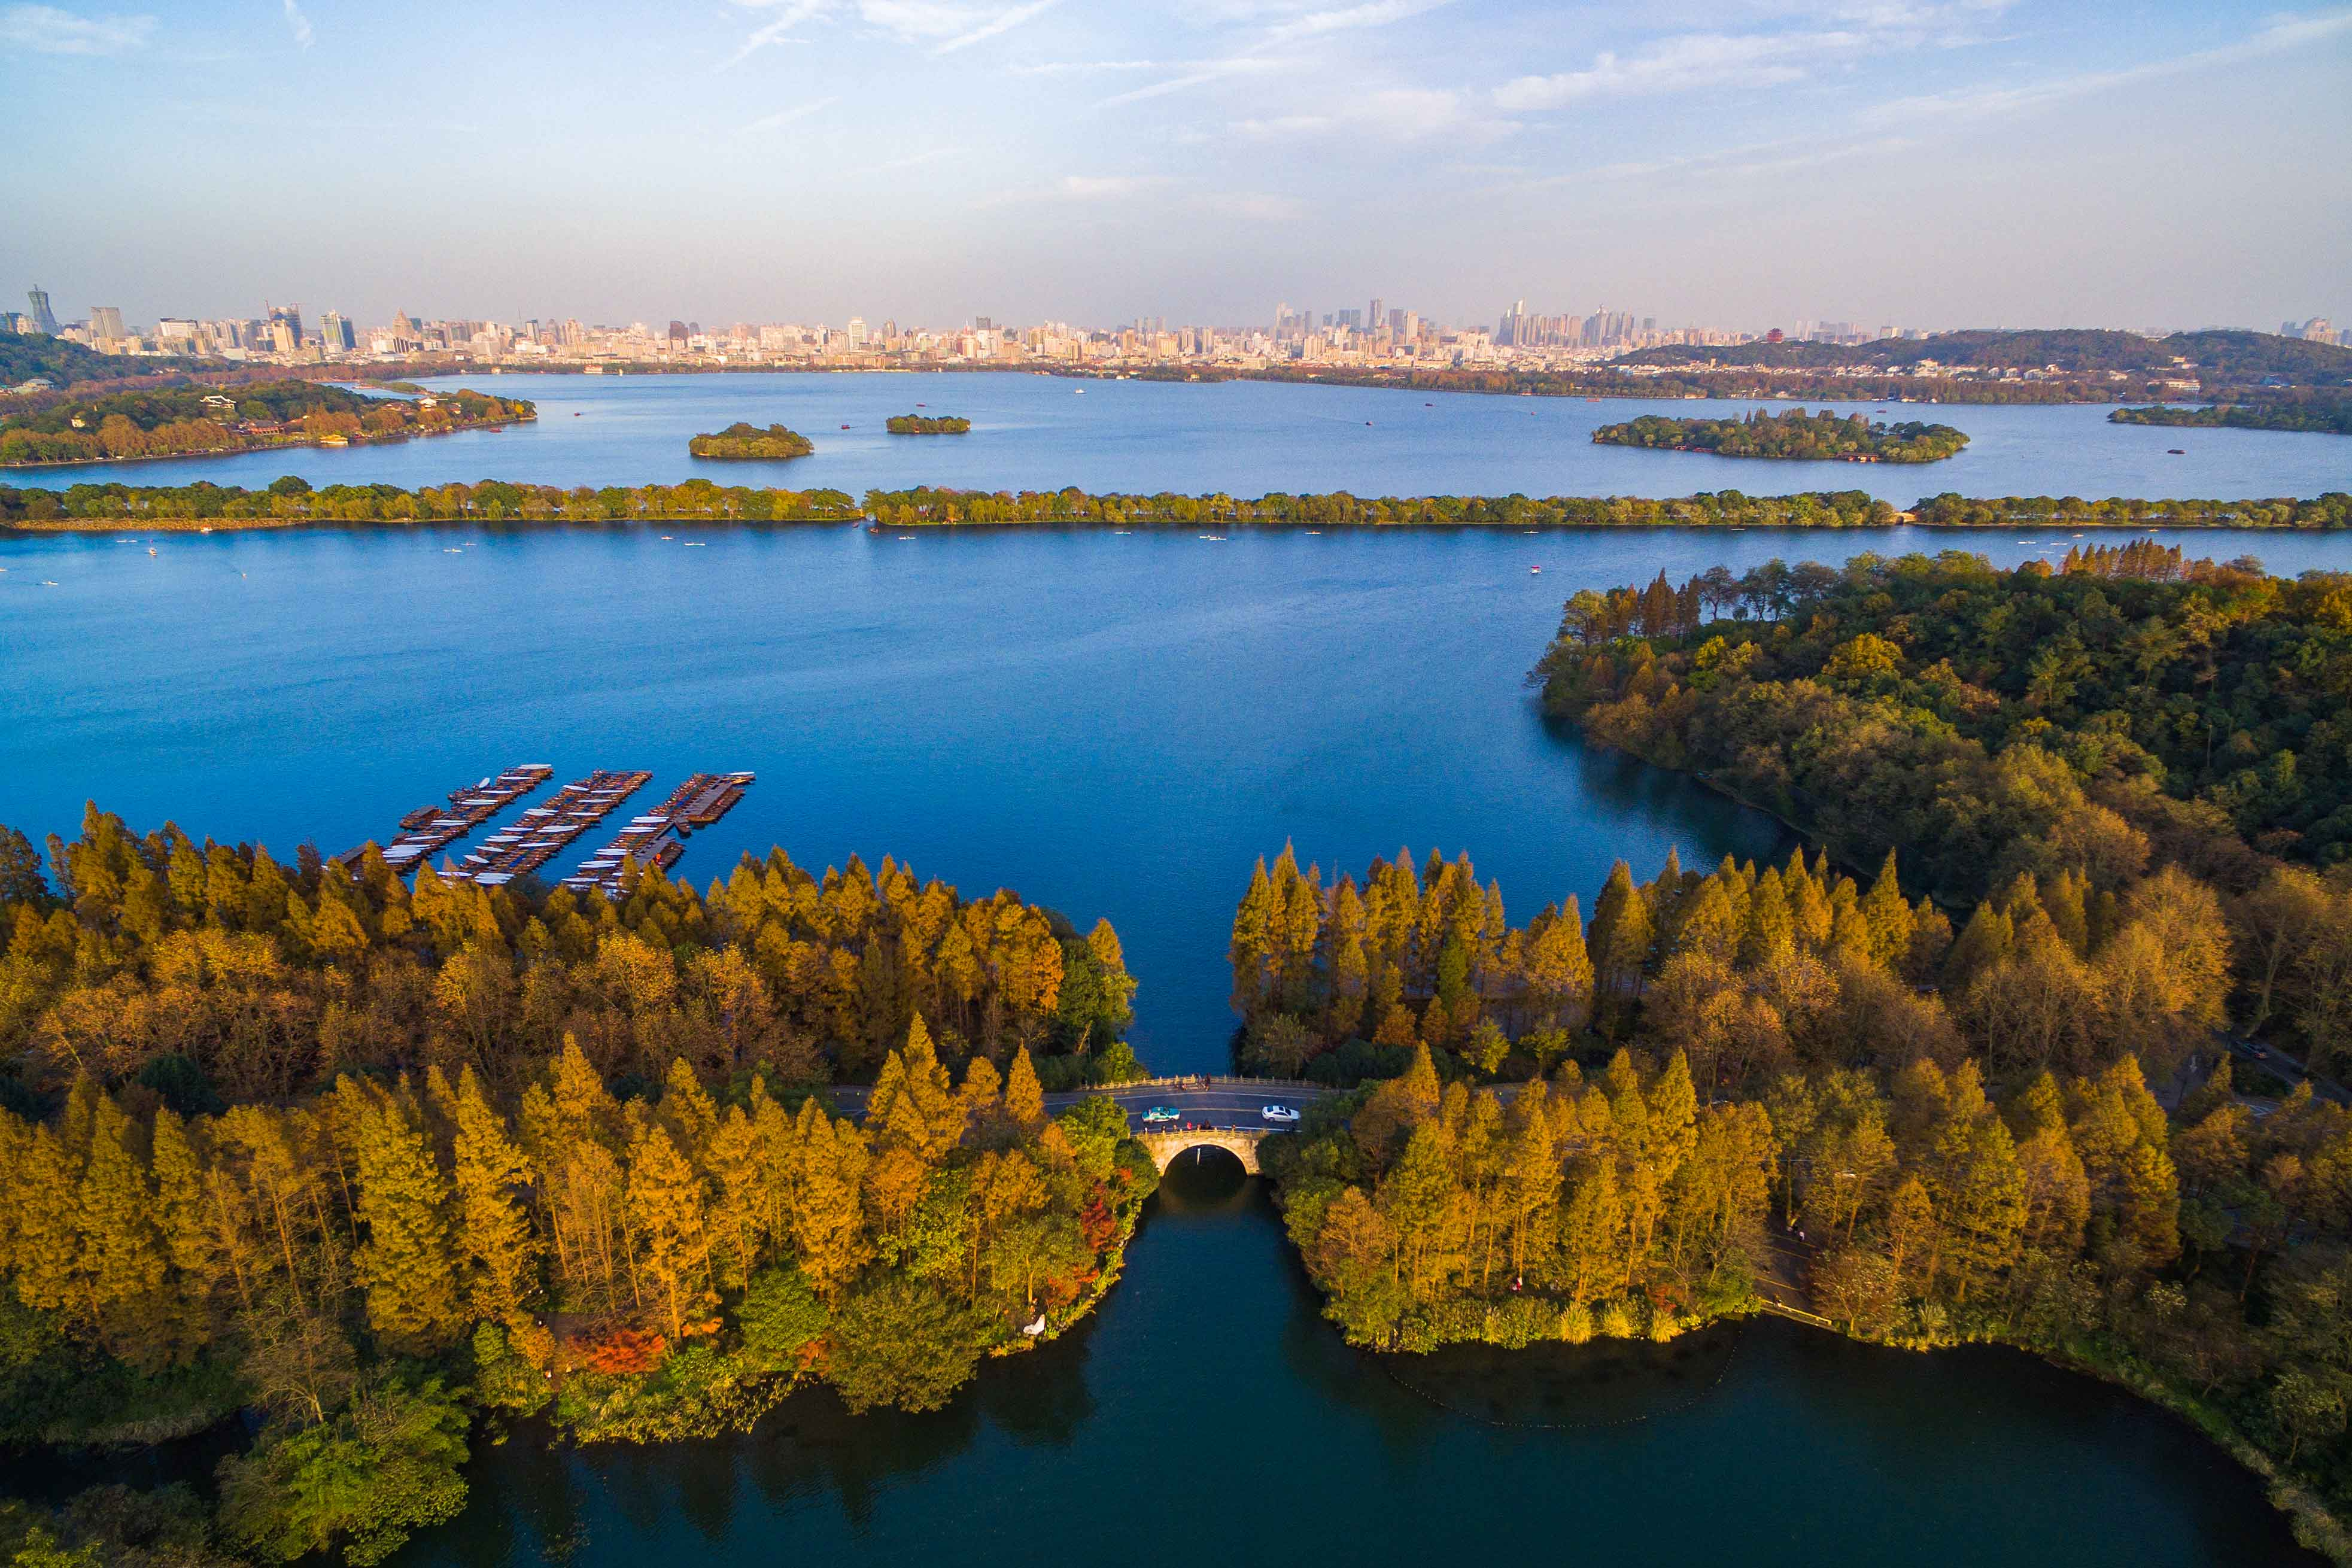
\includegraphics[scale=0.045]{4.jpg} \label{5}
  }
  \quad
  \subfigure[Example two]{
  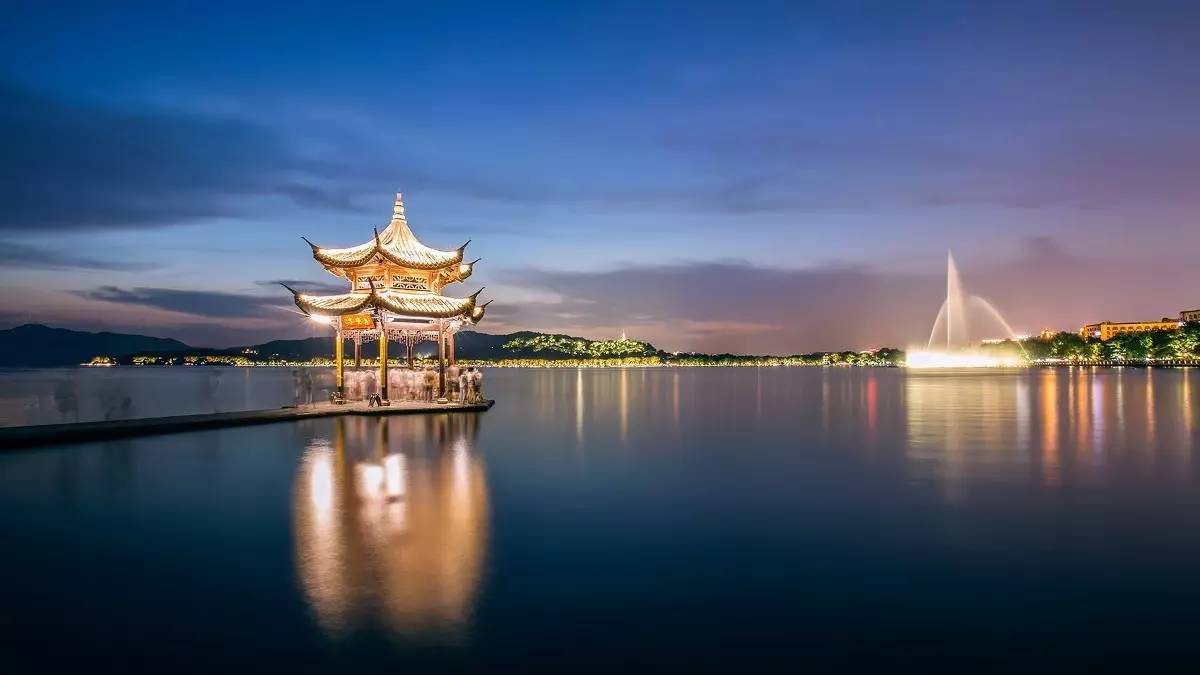
\includegraphics[scale=0.15]{5.jpg} \label{6} 
  }
  
  \caption{Experimental results of the author}
  \end{figure}
\subsection{研究目的}
为各位朋友提供出行攻略,使大家在被自控原理、嵌入式、小车、debug、程序设计以及
浴火重生的期中期末考试周中,有一个休息的时刻
\subsection{研究意义}
在繁忙的考试周中,给大家提供一个放松的休息时刻是非常重要的。在杭州旅游中,
除了可以欣赏美丽的西湖和探索古老的灵隐寺外,还可以品尝当地的特色美食,
购物体验等等。杭州作为一座历史悠久的城市,拥有丰富的历史文化和传统手工艺,可以让人领略到不同的风土人情
\subsection{文献综述}
\subsubsection{国内外文献综述}
国内文献综述:

一.杭州市旅游休闲业发展规划

该规划由杭州市人民政府发布,详细规划了杭州市在旅游休闲业方面的发展目标和措施,为杭州旅游业的发展提供了重要的指导。

二.饮食旅游动机对游客满意度和行为意向的影响研究

该研究探讨了饮食在旅游中的重要性,分析了饮食对游客满意度和行为意向的影响,为了解杭州饮食文化在旅游中的作用提供了参考。

三.地方饮食文化的挖掘及旅游开发研究

该研究探讨了地方饮食文化的挖掘和旅游开发,分析了饮食文化对旅游发展的影响,为杭州地方饮食文化的传承和发展提供了思路。

国外文献综述:

One.The Impact of Gastronomy Tourism on Tourist Satisfaction and Behavioral Intentions

This study explores the importance of gastronomy in tourism, a
nalyzing the impact of gastronomy on tourist satisfaction and behavioral intentions. It 
provides insights into the role of gastronomy in tourism, which can be applied to understa
nd the influence of Hangzhou's gastronomy culture on tourism.

Two.Cultural Tourism Development through Culinary Heritage

This research discusses the development of cultural touri
sm through culinary heritage, examining how culinary culture contributes to tourism develop
ment. It offers perspectives on how Hangzhou's culinary heritage can be leveraged for tourism promotion.
Culinary Tourism and Local Economic Development

This study investigates the relationship between 
culinary tourism and local economic development, highlighting the economic benefits of promoting culinary tourism. It sheds light on the potential economic impact of Hangzhou's culinary tourism on the local economy.

通过对国内外文献的综合分析,可以更全面地了解杭州旅游的吸引力及其影响因素,为研究提供理论支持和参考依
据。根据不同文献的观点和结论,可以进一步深入研究杭州旅游发展的策略和措施。



\section{数据预处理}
\subsection{数据采集}
为保证数据的可靠性,数据都由作者本人获得。以下图片以及言论均来自ZJU人群,主要取得途径:朵朵、CC98。

采集的数据包括学生的出行偏好、旅游目的地选择因素、旅游消费习惯等信息。当然,我们主要关注学生中好笑的事情。

\begin{figure}[H]
  \centering
  \subfigure[Proof one]{
  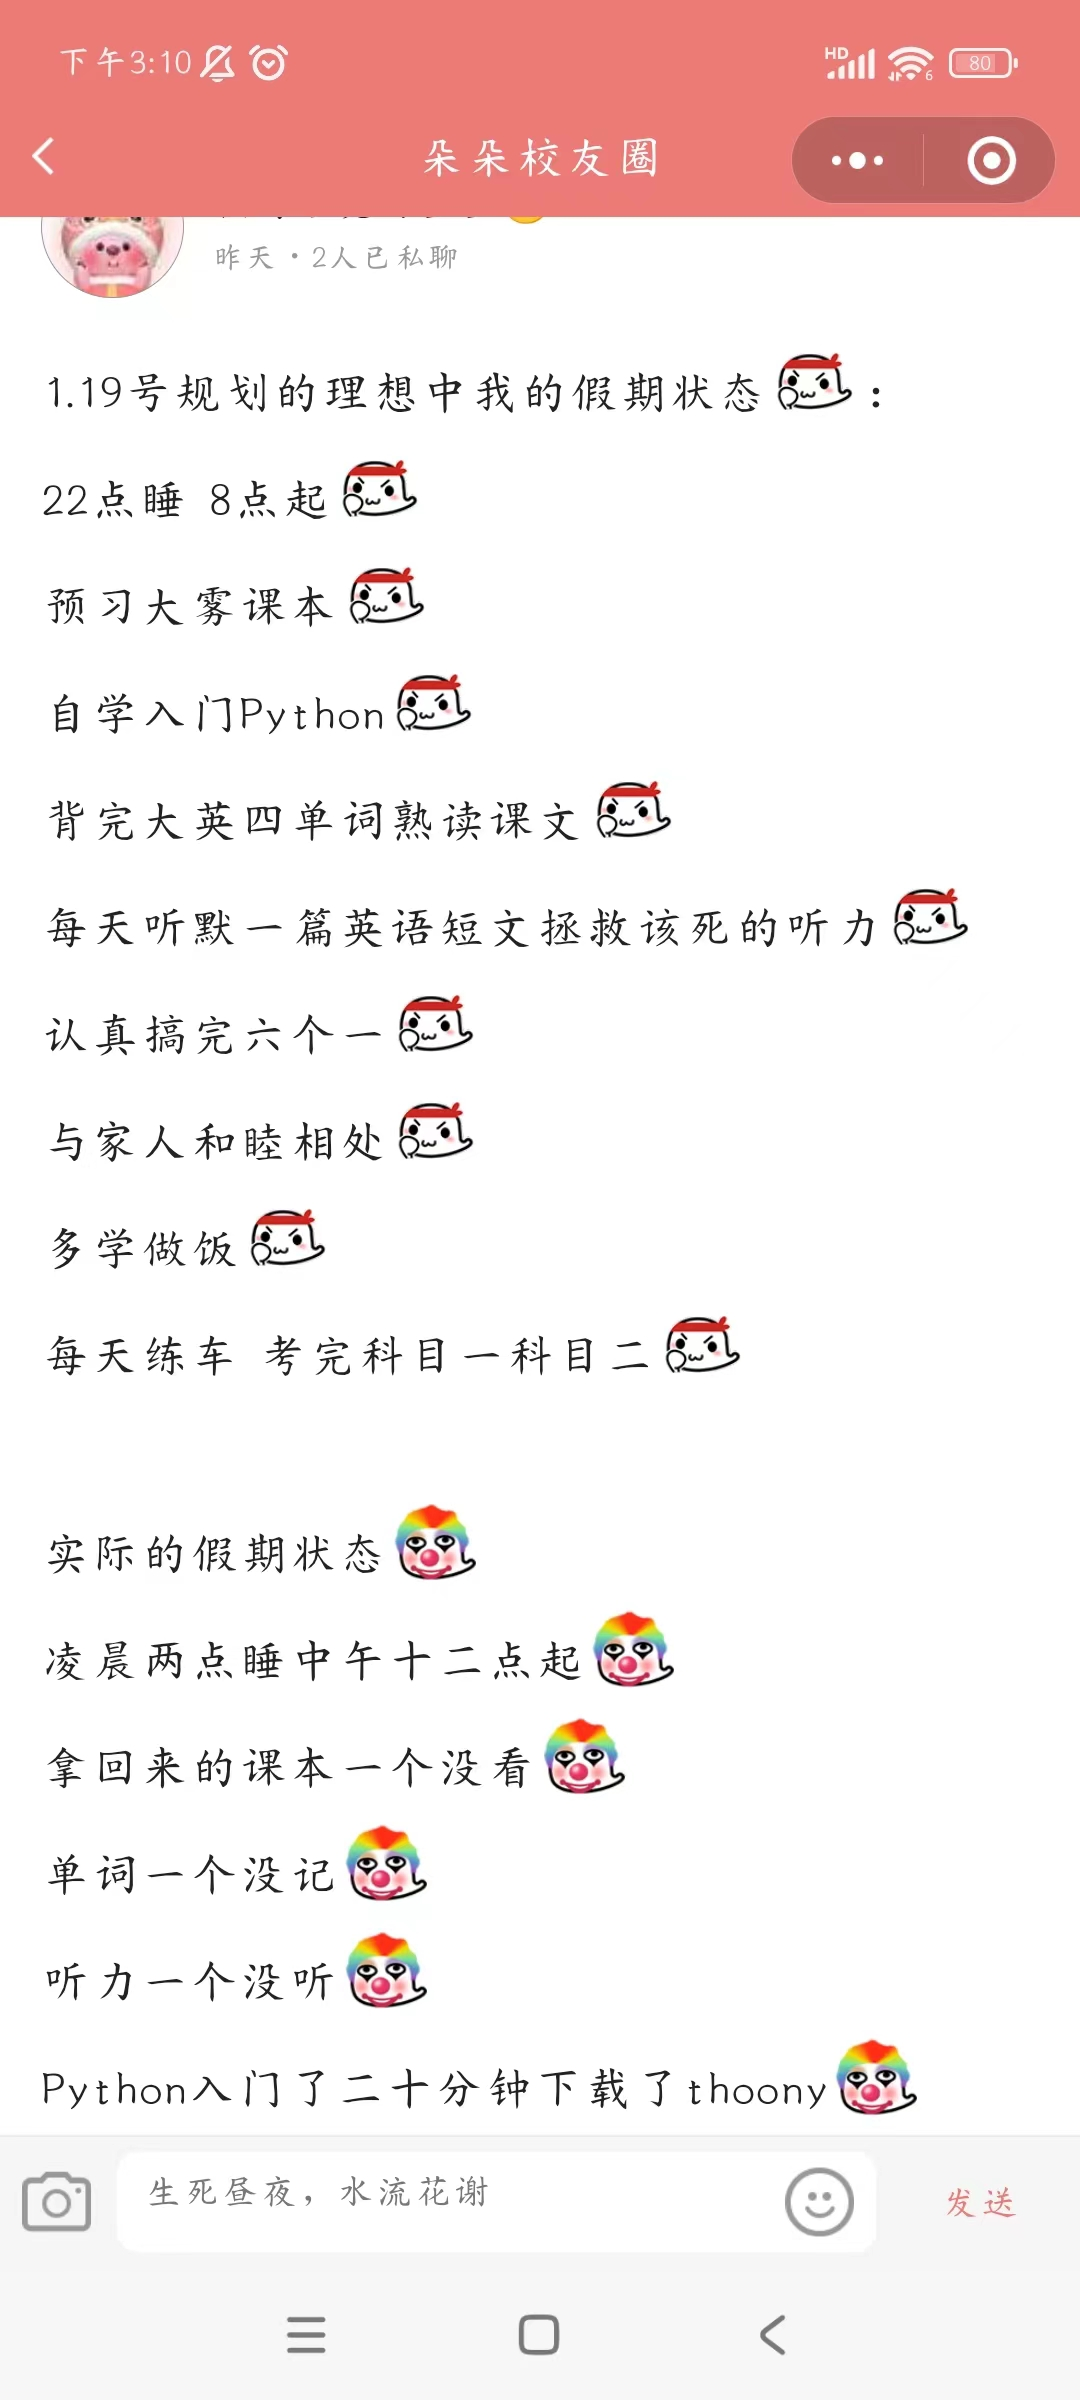
\includegraphics[scale=0.1]{3.jpg} \label{3}
  }
  \quad
  \subfigure[Proof two]{
  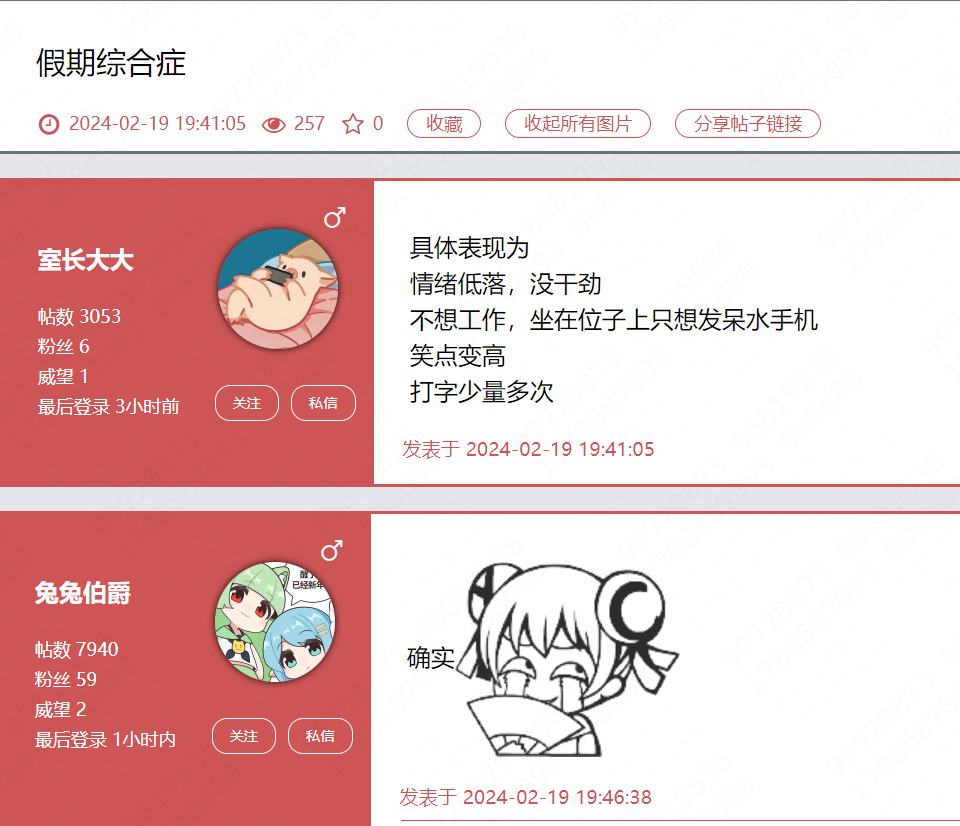
\includegraphics[scale=0.4]{4.png} \label{4} 
  }
  
  \caption{Experimental results of the author}
  \end{figure}

  从中我们可以看出,只是学习或做题是不好滴。
\subsection{数据预处理}

在数据预处理阶段,首先对采集到的数据进行清洗和整理,包括去除重复数据、处理缺失值、统一数据格式等操作。然后进行数据转换和标准化,
以便进行后续的分析和建模。最后,对数据进行探索性分析,了解数据的分布特征和相关性,为指标构建和分析提供基础。

\section{指标的构建}
\subsection{变量探索性分析}
通过对数据进行探索性分析,可以了解不同变量
之间的关系和特征。可以对不同变量进行描述性统计分析,绘制相关图表,探讨其分布情况和变化趋势。
\subsection{变量筛选}
在变量筛选阶段,根据探索性分析的结果和研究目的,筛选出对研究问题具有重要影响的变量。可以通过相关性分析、回归分析等方法,确定最终的研究指标,并进行进一步的建模和分析。

通过以上数据处理步骤,可以更深入地了解杭州旅游目的地选择的影响因素和规律,为研究提
供可靠的数据基础和分析结果。这些数据处理过程将有助于揭示学生出游行为背后的动机和因素,为后续研究提供重要参考。

首先,休息影响学习效果。休息影响个体的记忆保持量(Martini et al., 20
18; Martini et al., 2018; Martini et al., 2020; Martini et al., 2019)。

被试在两种条
件下完成两个单词列表的记忆任务,第一步,记忆第一个单词列表;第二步,立即回忆该列表中的单词;第三步,被试要
么进行休息,要么完成分心任务;第四步,记忆第二个单词列表;第五步,回忆该列表中的单词;第六步,被试要么进行
休息,要么完成分心任务;最后,完成自由回忆测试。结果表明,休息后的记忆保持量比分心后的保持量更大(Ma
rtini et al., 2018a,b, 2019)。休息的作用
与睡眠的作用相似,个体在睡眠后的记忆保持量更大(Backhaus et al., 2008)
。Ellenbogen等人 (2006)认为,这是因为睡眠保护暂时的记忆痕迹免受干扰的破坏性影响造成的结果。

\noindent{\textbf{\zihao{4}【致谢】}}

首先,感谢浙江大学这么早就让我们返回学校,让我们在这“温暖”的杭州内有时间分析。

其次,要感谢我的老师们,是他们,一次次钉钉中“你已被邀请入群聊”的消息,提醒着我,你的假期结束了。
正是那些睿智的老师们,布置下那计划学生很快完成的课后作业、大作业以及随堂测试,让我们生活快乐且充实。

最后,更要感谢身边的人们,没有你们,我都不会知道这么多有趣的事情。

\noindent{\textbf{\zihao{4}【参考文献】}}


[1] 杭州市人民政府办公厅关于印发杭州市旅游休闲业发展“十三五”规划的通知[J]. .杭州市人民政府公报,2016(S1)

[2] 饮食旅游动机对游客满意度和行为意向的影响研究[J]. 张涛.旅游学刊,2012(10)

[3] 我国饮食文化旅游开发研究[J]. 朱晓翔.江苏商论,2008(10)

[4] 地方饮食文化的挖掘及旅游开发研究[J]. 黄莉.现代食品,2019

[5] 饮食文化对旅游发展的影响[J]. 何宏.社会科学战线,2007

[6] 旅游影响下的地方饮食文化生产转向:特征与机制[J]. 侯兵;李红缘;余凤龙;张爱平.旅游学刊,2024

[7] 认知灵活性、认知坚持性对学习效率的影响——工作记忆容量的调节作用[J].胡彦兰

[8] 中学生厌学心理及其干预与学习效率的相关研究[J].傅安球;聂晶;李艳平;金蓓蓓;崔君红 心理科学
\addcontentsline{toc}{section}{参考文献}\tolerance=500 
\addcontentsline{toc}{section}{致谢}\tolerance=500
\end{document}
